\chapter{Desenvolupament del projecte}
En aquest capítol s'explicarà el funcionament del programa, es mostrarà com s'ha donat solució a cada un dels requeriments plantejats a l'apartat de disseny, es descriurà el procés de proves que s'ha realitzat per assegurar la qualitat del programari i la forma d'exportar el projecte a fitxers executables per l'usuari final.
%-----------------------------------------------------------------------
\section{Conceptes que s'han de conèixer}
\subsection{Què és Spring Boot?}
Per al desenvolupament del backend, s'ha utilitzat el framework Spring Boot. Spring Boot és una eina de desenvolupament de programari lliure basada en Java. Facilita la creació d'aplicacions Java de qualitat de forma senzilla i ràpida. Aprofita el poder de l'ecosistema Spring però redueix la necessitat de configuració i personalització.
\\[3mm]
Spring Boot s'utilitza per construir aplicacions Java autònomes, és a dir, aplicacions que no requereixen un servidor web separat per a funcionar. Això és possible gràcies al seu suport per a contenidors integrats. Aquesta característica permet que l'aplicació s'executi com un fitxer JAR amb un servidor web incorporat, com ara Tomcat o Jetty.
\\[3mm]
Una altra característica clau de Spring Boot són els "starters". Els "starters" són conjunts de dependències que simplifiquen la configuració inicial d'una aplicació. Proporcionen configuracions predeterminades per a casos d'ús comuns, com ara aplicacions web o accés a bases de dades. Amb l'ús dels "starters", es pot començar a desenvolupar una aplicació amb les dependències adequades amb poques línies de codi.
\\[3mm]
Spring Boot també ofereix una funcionalitat d'autoconfiguració. Utilitza tècniques de programació reflexiva per analitzar les llibreries i classes disponibles en l'aplicació i configura automàticament els components segons les necessitats detectades. Això evita haver de realitzar configuracions manuals i permet als desenvolupadors centrar-se en la lògica de l'aplicació en lloc de preocupar-se per la configuració tècnica.
\\[3mm]
Amb Spring Boot, és fàcil desenvolupar aplicacions RESTful, gestionar peticions web, interactuar amb bases de dades, implementar seguretat, programar tasques i integrar-se amb sistemes de missatgeria.
\\[3mm]
En resum, Spring Boot és una eina que simplifica el desenvolupament d'aplicacions Java, permetent als desenvolupadors crear aplicacions de qualitat de forma senzilla i ràpida. Amb el seu suport per a contenidors integrats, els "starters" i la funcionalitat d'autoconfiguració, Spring Boot redueix la complexitat i la necessitat de configuració, permetent als desenvolupadors centrar-se en la creació de lògica d'aplicacions.
\subsection{Programació reactiva: WebFlux, fluxos de dades i l'efecte Hollywood}
La programació d'API Reactiva és un enfocament per a construir APIs que abraça els principis reactius. La programació reactiva és un paradigma de programació que es centra en la programació asíncrona i basada en esdeveniments, permetent que els sistemes siguen més responsius, escalables i resistents. En el context de les APIs, la programació reactiva permet gestionar un gran nombre de sol·licituds concurrents amb un nombre reduït de fils d'execució, millorant així l'aprofitament dels recursos i reduint les operacions de bloqueig.
\\[3mm]
Spring WebFlux és un framework proporcionat per l'ecosistema de Spring. Està dissenyat per a donar suport a models de programació reactius, incloent fluxos de dades (o streaming) i entrada/eixida no bloquejant. Spring WebFlux permet als desenvolupadors construir endpoints d'API reactius aprofitant la llibreria \href{https://projectreactor.io/}{Reactor}. Aquests endpoints són notificats i invocats pel framework quan arriben sol·licituds, seguint un model basat en esdeveniments. Aquesta inversió de control és similar a l'"efecte Hollywood", on el framework assumeix el comandament i crida els controladors adequats quan siga necessari.
\\[3mm]
Ara, abordem la relació entre l'"efecte Hollywood" i la programació d'API Reactiva amb Spring WebFlux. Encara que no hi ha una connexió directa entre els dos conceptes, podem fer una analogia per a entendre'ls millor. L'efecte Hollywood, conegut també com "No ens crides, ja te cridarem nosaltres", és un principi que s'aplica en la programació reactiva i es refereix a invertir la direccionalitat de les sol·licituds. Segons aquest principi, el client no farà trucades periòdiques al servidor per a saber si ha ocorregut o no un esdeveniment, sinó que es subscriurà a un endpoint i en el que el servidor anirà publicant dades quan corresponga.
\begin{figure}[H]
    \centering
    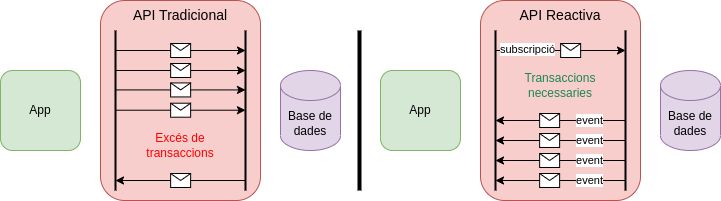
\includegraphics[width=\textwidth]{images/reactiva.png}
    \caption{Programació reactiva}
    \label{fig:Programació reactiva}
\end{figure}
\noindent
Des de el punt de vista del codi, per a crear un servici que publique dades a un endpoint reactiu utilitzant Spring
WebFlux s'ha d'especificar que aquest generarà dades del tipus "TEXT\_EVENT\_STREAM\_VALUE" i s'ha d'utilitzar la classe Flux de la següent manera:
\begin{minted}[fontsize=\footnotesize]{java}
@GetMapping(
    path = "/path/to/endpoint",
    produces = MediaType.TEXT_EVENT_STREAM_VALUE
)
public Flux<List<Object>> stream() {
    return Flux.just(repository.getAll());
}
\end{minted}
Per a subscriure's des de TypeScript s'utilitza la classe EventSource d'aquesta forma:
\begin{minted}[fontsize=\footnotesize]{typescript}
let stream = new EventSource("/path/to/endpoint");
stream.onmessage = (event) => {
    /* Funció a executar */
}
\end{minted}
%-----------------------------------------------------------------------
\section{Estructura i processos}
A aquest apartat s'aprofundirà en l'estructura i fluxos d'execució del codi.
\\[3mm]
Encara que el projecte compta amb diferents mòduls, només s'abordaran l'estructura i processos del backend, ja que és ací on es pot observar una arquitectura més clara i interessant, la resta del codi són fitxers TypeScript que realitzen tasques espontànies al frontend i gestionen peticions HTTP.
\subsection{Estructura de classes}
El backend es pot desgranar en dos parts diferenciades; l'API que s'encarrega de les comunicacions i fer les tasques pròpies d'un servidor, i el motor d'escacs, que s'encarrega de la lògica del joc.
\\[3mm]
Per a interactuar correctament amb Spring Boot s'han d'anotar les classes com a components (concepte similar a model, vista i controlador), existeixen principalment quatre tipus:
\begin{enumerate}
    \item Entitat: és una classe POJO (Plain Old Java Object) i representa una taula en la capa de persistència de dades
    \item Controlador: el seu propòsit principal és gestionar les peticions HTTP entrants i retornar respostes adequades, és responsable de definir els punts d'entrada de l'aplicació web, coneguts com a endpoints.
    \item Servici: és una classe que conté la lògica de negoci i s'encarrega de coordinar les diferents operacions dins de l'aplicació, proporcionant una capa d'abstracció entre els controladors i la capa de persistència de dades.
    \item Repositori: és una interfície o classe que proporciona una abstracció per accedir a les dades de l'aplicació i realitzar operacions de persistència, eliminant la complexitat de les operacions de baix nivell i permetent una interacció més senzilla i escalable amb la capa de persistència de dades.
\end{enumerate}
A banda, s'han escrit excepcions personalitzades per a cada tipus d'error i un gestor global per a aquestes, així com classes utilitàries per a encriptació, seguretat o configuració.
\begin{figure}[H]
    \centering
    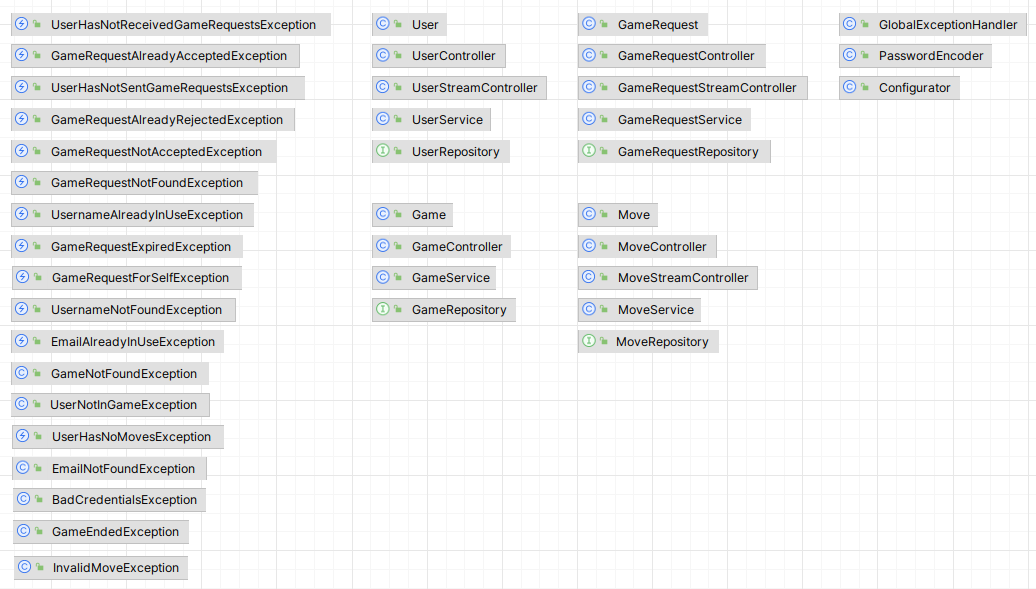
\includegraphics[width=\textwidth]{images/api.png}
    \caption{Diagrama de classes de l'API}
    \label{fig:Diagrama de classes de l'API}
\end{figure}
\noindent
El motor utilitza classes convencionals, que no interactuen amb el framework Spring Boot, es pot observar els diferents tipus de peces i l'herència que comparteixen amb la classe pare, així com classes de presència pràcticament obvia a un motor d'escacs, per exemple la classe tauler o casella. També trobem classes útils per a traduir informació a objectes de Java, s'aprofundirà més en aquest aspecte a la \hyperref[sec:engine]{secció d'implementació d’un “chess engine”}.
\begin{figure}[H]
    \centering
    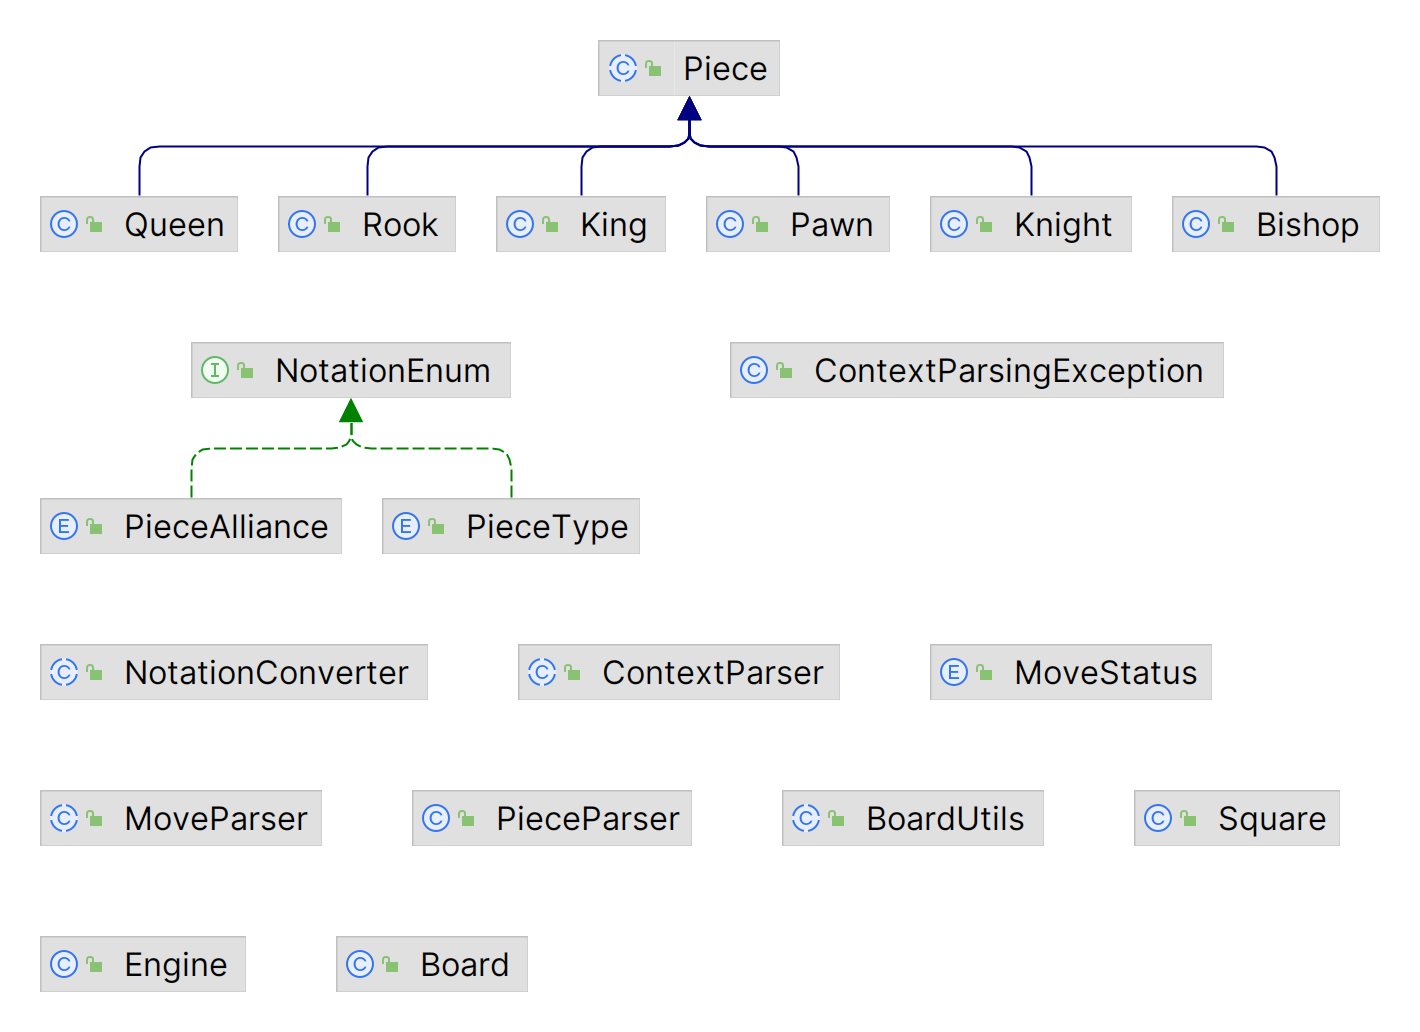
\includegraphics[width=0.8\textwidth]{images/engine.png}
    \caption{Diagrama de classes del motor}
    \label{fig:Diagrama de classes del motor}
\end{figure}
\subsection{Flux d'execució normal}
En la majoria dels casos, el flux d'execució de les peticions consta dels següents passos:
\begin{enumerate}
    \item L'usuari interactua a través del frontend i es genera una sol·licitud HTTP.
    \item La sol·licitud aplega al endpoint d'un controlador, aquest la gestiona i la passa al servici que corresponga.
    \item El servici realitza alguna acció amb la informació rebuda, cridarà al motor d'escacs o a la base de dades si és necessari i comunicarà el resultat al controlador del pas anterior.
    \item El controlador generarà una resposta HTTP i contestarà al client.
\end{enumerate}
\begin{figure}[H]
    \centering
    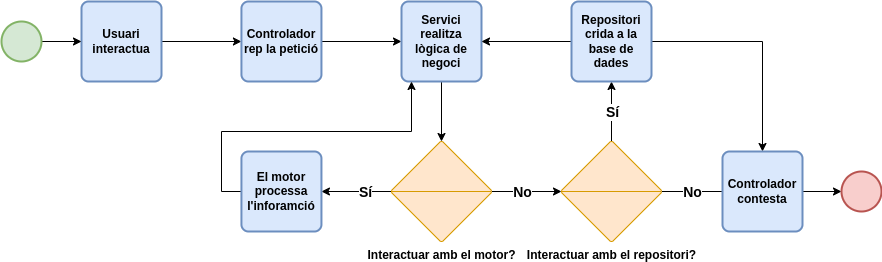
\includegraphics[width=\textwidth]{images/fluxe.png}
    \caption{Flux d'execució normal}
    \label{fig:Flux d'execució normal}
\end{figure}
%-----------------------------------------------------------------------
\section{Codificació}
Es detallarà en profunditat com s'ha abordat i resolt cadascun dels requeriments establerts en l'apartat de disseny. Es descriurà el procés i les estratègies utilitzades per garantir que cada requeriment s'ha complit de manera efectiva i satisfactòria. A més, es proporcionaran exemples concrets i evidències de com s'han implementat les solucions per a cada requeriment, mostrant la seva contribució a la qualitat general del programari.
\subsection{Sistema de registre}
El registre consisteix en la validació i creació d'un nou usuari a partir de les dades que s'introdueixen al formulari de registre.
\\[3mm]
Quan un usuari plena el formulari amb les dades que es sol·liciten i fa clic al botó d'enviar els camps del formulari es tradueixen a format JSON i s'envia una petició HTTP de tipus POST al servidor, aquest és l'encarregat de processar-la i tornar feedback al frontend.
\\[3mm]
En primer lloc es du a terme una validació les dades, per a açò s'utilitza tant Spring Validation com codi propi de l'aplicació. Per part de Spring Validation, s'utilitzen funcionalitats per a comprovar que ningun dels camps introduïts estan buits, també es comprova que el correu electrònic compleix els requisits definits a una expressió regular, aquest ha de contindre elements com l'arrova (@) o un domini (.com, .es) i nomes podrà contindre caràcters alfanumèrics. Després es fan consultes a la base de dades per a assegurar-se de que el nom d'usuari i el correu electrònics són únics a l'aplicació.
\\[3mm]
Una vegada validat, s'ha d'inserir l'usuari a la base de dades, per a fer-ho de forma segura, abans s'encripta la contrasenya mitjançant funcions criptogràfiques presents al paquet \href{https://docs.oracle.com/javase/7/docs/api/javax/crypto/package-summary.html}{javax.crypto}, en concret s'utilitza el algoritme de hash PBKDF2.
\\[3mm]
Finalment, el servidor tornarà feedback al client, si els passos anteriors s'han executat satisfactòriament, rebrà la informació referent al nou usuari registrat, en cas contrari rebrà un missatge d'error amb la descripció d'aquest. Aquesta resposta es veurà reflectida al formulari, si és favorable es permetrà l'accés, però si no és així es mostrarà una alerta amb la descripció del problema.
\\[3mm]
És important destacar que s'utilitza la \href{https://github.com/FasterXML/jackson}{API Jackson} per a amagar la contrasenya del usuari, de manera que mai s'enviarà a través de la xarxa (encara que prèviament ha segut encriptada).
\subsection{Sistema d'inici de sessió}
Aquest sistema rep les credencials que s'introdueixen al formulari d'inici de sessió i les contrasta amb les que es troben a la base de dades.
\\[3mm]
Comparteix característiques amb l'apartat anterior, per exemple el procés de validació es molt semblant i utilitza les mateixes funcions. La principal diferència la trobem a l'hora de comprovar si la contrasenya introduïda (que serà text plà) coincideix amb la que hi ha al sistema (que estarà encriptada), per a açò s'utilitza un procés d'enginyeria inversa, s'encripta amb el mateix algoritme que s'havia utilitzat al registre i es comparen byte per byte. D'aquesta forma mai s'intenten desencriptar les credencials que ja consten a la base de dades.
\\[3mm]
Per últim, novament de forma similar a l'apartat anterior, el servidor contesta al client i es produeixen els canvis necessaris.
\subsection{Sistema d'emparellament}
Per a emparellar-se, els jugadors han de poder enviar i rebre sol·licituds de joc, per tant podem diferenciar dos rols, el d'emissor i el de receptor.
\\[3mm]
Els jugadors registrats a l'aplicació apareixeran a un llistat, des de ací l'usuari emissor podrà seleccionar al receptor i enviar-li una sol·licitud a la seua bústia, que es troba a la pàgina de sol·licituds. En realitat la bústia es una tabla (HTML) subscrita a un endpoint reactiu, on el servidor publica mitjançant un flux de dades les sol·licituds pendents dels usuaris que ho consulten, i que s'actualitza cada vegada que hi ha alguna novetat. Es considera que una sol·licitud està pendent quan no ha expirat ni ha segut acceptada o rebutjada.
\\[3mm]
En aquest apartat observem un exemple de l'ús de la programació reactiva, tant en la tabla d'usuaris com en la de sol·licituds de joc, ja que aquestes s'actualitzen automàticament quan ocorre algun event als endpoints als que estan subscrites, si s'hagués utilitzat el paradigma tradicional es tindria que haver incorporat un botó per a refrescar-les, augmentant la quantitat de peticions al servidor i a la base de dades.
\subsection{Implementació d’un “chess engine”}
\label{sec:engine}
El motor d’escacs funciona com una “caixa negra” en la que el servidor executa les jugades que rep dels clients, aquestes jugades s'envien en format "portable game notation", per tant s'ha d'extraure la informació i transformar-les en objectes Java per a poder ser analitzades.
\\[3mm]
La notació de joc portàtil d'escacs, coneguda com a "Portable Game Notation" (PGN), és una forma estandarditzada d'enregistrament de partides d'escacs, els seus moviments i informació relacionada. Permet compartir, analitzar i emmagatzemar les partides d'escacs utilitzant text pla. A més, el PGN permet afegir informació addicional com ara encapçalaments de partida, detalls de l'esdeveniment, noms dels jugadors i anotacions.
\\[3mm]
La notació PGN representa cada moviment amb una combinació del símbol de la peça i la casella de destí. Ací alguns exemples:
\begin{itemize}
    \item Moviments de peó: Els peons són representats pel seu símbol (sense lletra) i la casella de destí. Per exemple, e4 representa moure el peó a la casella e4.
    \item Moviments de peces: Les peces són representades per la seua lletra majúscula, seguida de la casella de destí. Per exemple, Nf3 representa moure un cavall a la casella f3.
    \item Captures: Les captures es denoten amb una 'x' entre el símbol de la peça i la casella de destí. Per exemple, Bxc5 representa un alfil capturant una peça en la casella c5.
    \item Enroc: L'enroc al costat del rei es representa amb la notació O-O, mentre que al costat de la reina s'indica amb O-O-O.
    \item Escac i escac i mat: '+' s'utilitza per indicar un escac, i '\#' s'utilitza per indicar escac i mat. Per exemple, Qh5+ representa una reina fent escac al rei oponent en la casella h5.
    \item Altres símbols: '=' s'utilitza per indicar una promoció de peó, i '!' i '?' s'utilitzen per a denotar moviments bons i dolents, respectivament.
\end{itemize}
Aquest sistema de notació és complex, per això, a aquest projecte s'ha implementat una versió simplificada i més fàcil d'interpretar de PGN.
\\[3mm]
Tornant al tema del motor d'escacs, aquest ha de ser capaç de reproduir el context del tauler i crear un objecte a partir d'aquesta informació, de manera que quan volem executar un moviment, no només haurem de proporcionar el seu valor, sinó també dades sobre l'estat de la resta de caselles i les peces que contenen.
\\[3mm]
Una vegada s'han proporcionat les dades, es transformaran en diferents instàncies d'objectes Java i es podrà analitzar el moviment, aquest estudi serà diferent per a cada tipus de peça. Al joc trobem sis tipus diferents, que hereten d’una classe superior. La principal diferència entre aquestes es troba als moviments vàlids que poden realitzar, tenint en compte les normes del joc, s’han d’implementar aquests comportaments de forma individual per a cada peça. Quan es tracta del comportament de les peces, les podem dividir en dos grups; les que es mouen de forma vectorial i les que no.
\begin{itemize}
    \item Comportament vectorial: Aquestes peces es desplacen seguint la direcció d’un vector fins que es troben amb altra peça o amb el límit del tauler, bé siga en direcció dels punts cardinals (nord, sud, est, oest) o formant diagonals. En aquest grup trobem a les torres, els alfils i la reina.
    \item Comportament no vectorial: Aquestes peces tenen un rang de moviment definit per desplaçaments fixes o “offsets” partint de la posició en la que es troben, per exemple el rei es pot moure utilitzant els desplaçaments [-9, -8, -7, -1, 1, 7, 8, 9]. En aquest grup trobem els cavalls, els peons i el rei.
\end{itemize}
\begin{figure}[H]
     \centering
     \begin{subfigure}[b]{0.3\textwidth}
         \centering
         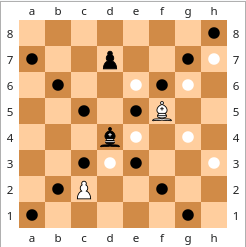
\includegraphics[width=\textwidth]{images/alfil.png}
         \label{fig:Alfil}
     \end{subfigure}
     \hspace{0.25\textwidth}
     \begin{subfigure}[b]{0.3\textwidth}
         \centering
         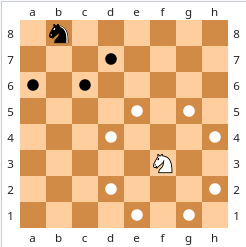
\includegraphics[width=\textwidth]{images/cavall.png}
         \label{fig:Rei}
     \end{subfigure}
        \caption{Exemples de desplaçament vectorial i no vectorial}
        \label{fig:Desplaçament vectorial i no vectorial}
\end{figure}
Tenint el compte el tipus de peça, es comprovarà el moviment, si és il·legal, no es podrà executar i es tornara un estatus d'error, però si és vàlid, es crearà un tauler "imaginari" a partir del que s'està analitzant, i en aquest s'executarà el moviment, d'aquesta manera podrem avaluar les conseqüències de la jugada sense alterar l'estat del tauler original, creant un mecanisme de "rollback". Després de dur a terme un moviment, poden passar tres coses:
\begin{enumerate}
    \item El moviment causa escac al rei contrari.
    \item El moviment causa escac i mat a l'oponent i per tant el fi de la partida.
    \item El moviment exposa al rei del jugador a escac, per tant el moviment s'ha de marcar com no vàlid.
\end{enumerate}
Per a saber si el rei està en escac, s'analitza cadascun dels moviments possibles de cadascuna de les peces de l'oponent, i es busquen aquells que tinguen com a casella de destinació la casella en la que està el rei. 
\\[3mm]
Per a calcular l'escac i mat, s'ha de complir, a més, que el rei no tinga cap moviment vàlid disponible, però també s'ha de comprovar si alguna de les peces pot cobrir el atac al rei, novament s'utilitza la mecànica del tauler "imaginari" per a computar aquests casos.
\subsection{Implementació d’una interfície gràfica d'usuari}
Es poden diferenciar tres tipus d'elements principals, que componen les distintes pàgines; els formularis, les taules i el tauler principal.
\\[3mm]
Per a les pàgines d'inici de sessió i registre, s'han fet servir formularis als quals s'ha modificat l'acció que fan quan s'envien (SubmitEvent) mitjançant un oient d'esdeveniments (EventListener), de manera que s'executa una funció personalitzada que transforma les dades introduïdes a format JSON i després utilitza l'API Fetch per a fer un POST al endpoint corresponent.
\\[3mm]
Després es processa la resposta del servidor i es mostra un missatge de benvinguda o d'error.
\begin{figure}[H]
     \centering
     \begin{subfigure}[b]{0.4\textwidth}
         \centering
         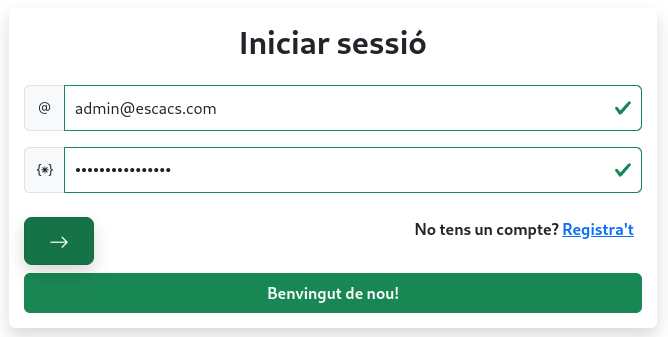
\includegraphics[width=\textwidth]{images/login-escacs.png}
         \label{fig:Login}
     \end{subfigure}
     \hspace{0.15\textwidth}
     \begin{subfigure}[b]{0.4\textwidth}
         \centering
         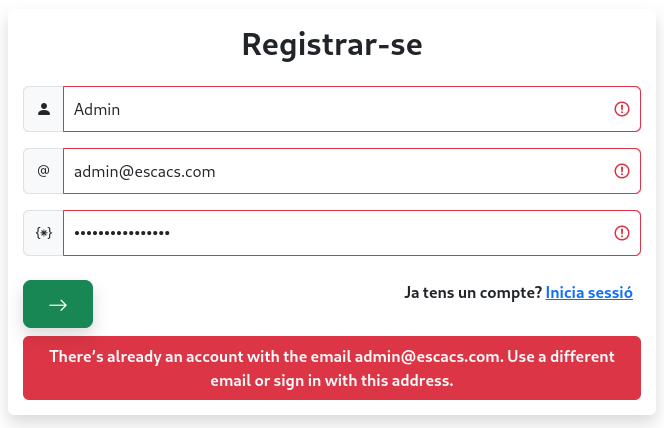
\includegraphics[width=\textwidth]{images/registre-escacs.png}
         \label{fig:Registre}
     \end{subfigure}
        \caption{Captures dels formularis d'inici de sessió i registre}
        \label{fig:Captures dels formularis d'inici de sessió i registre}
\end{figure}
\noindent
Quan l'usuari es valida al formulari d'inici de sessió, es motrarà la pàgina principal, que compta amb un tauler d'escacs i dues taules, una que mostra els moviments que es realitzen a la partida i altra que mostra els jugadors disponibles. D'aquesta pàgina és important destacar alguns aspectes, per exemple:
\begin{itemize}
    \item A la zona dreta de la barra superior es mostra el nom del usuari amb el que s'ha iniciat sessió.
    \item Al seleccionar una peça aliada al tauler, es pinten els moviments vàlids, així com els moviments d'atac, però no es mostrarà si es selecciona una peça del oponent. Açò s'aconsegueix mitjançant una consulta al servidor.
    \item Al llistat de moviments, es mostra el valor del moviment i la icona que correspon a la peça desplaçada, a més mostra els noms dels jugadors que participen a la partida.
    \item El llistat de jugadors es tracta d'una simplificació del tauler complet que es troba a la pàgina "Llistat de jugadors", també es pot accedir a aquest fent clic al botó blau que conté la icona de una lupa.
    \item Les alertes o missatges emergents es mostraran dalt de la barra superior. Es pot veure un exemple d'aquesta funcionalitat a la \hyperref[fig:Escac i mat]{figura d'escac i mat} que es troba a la secció "Resultat i conclusions finals".
\end{itemize}
\begin{figure}[H]
    \centering
    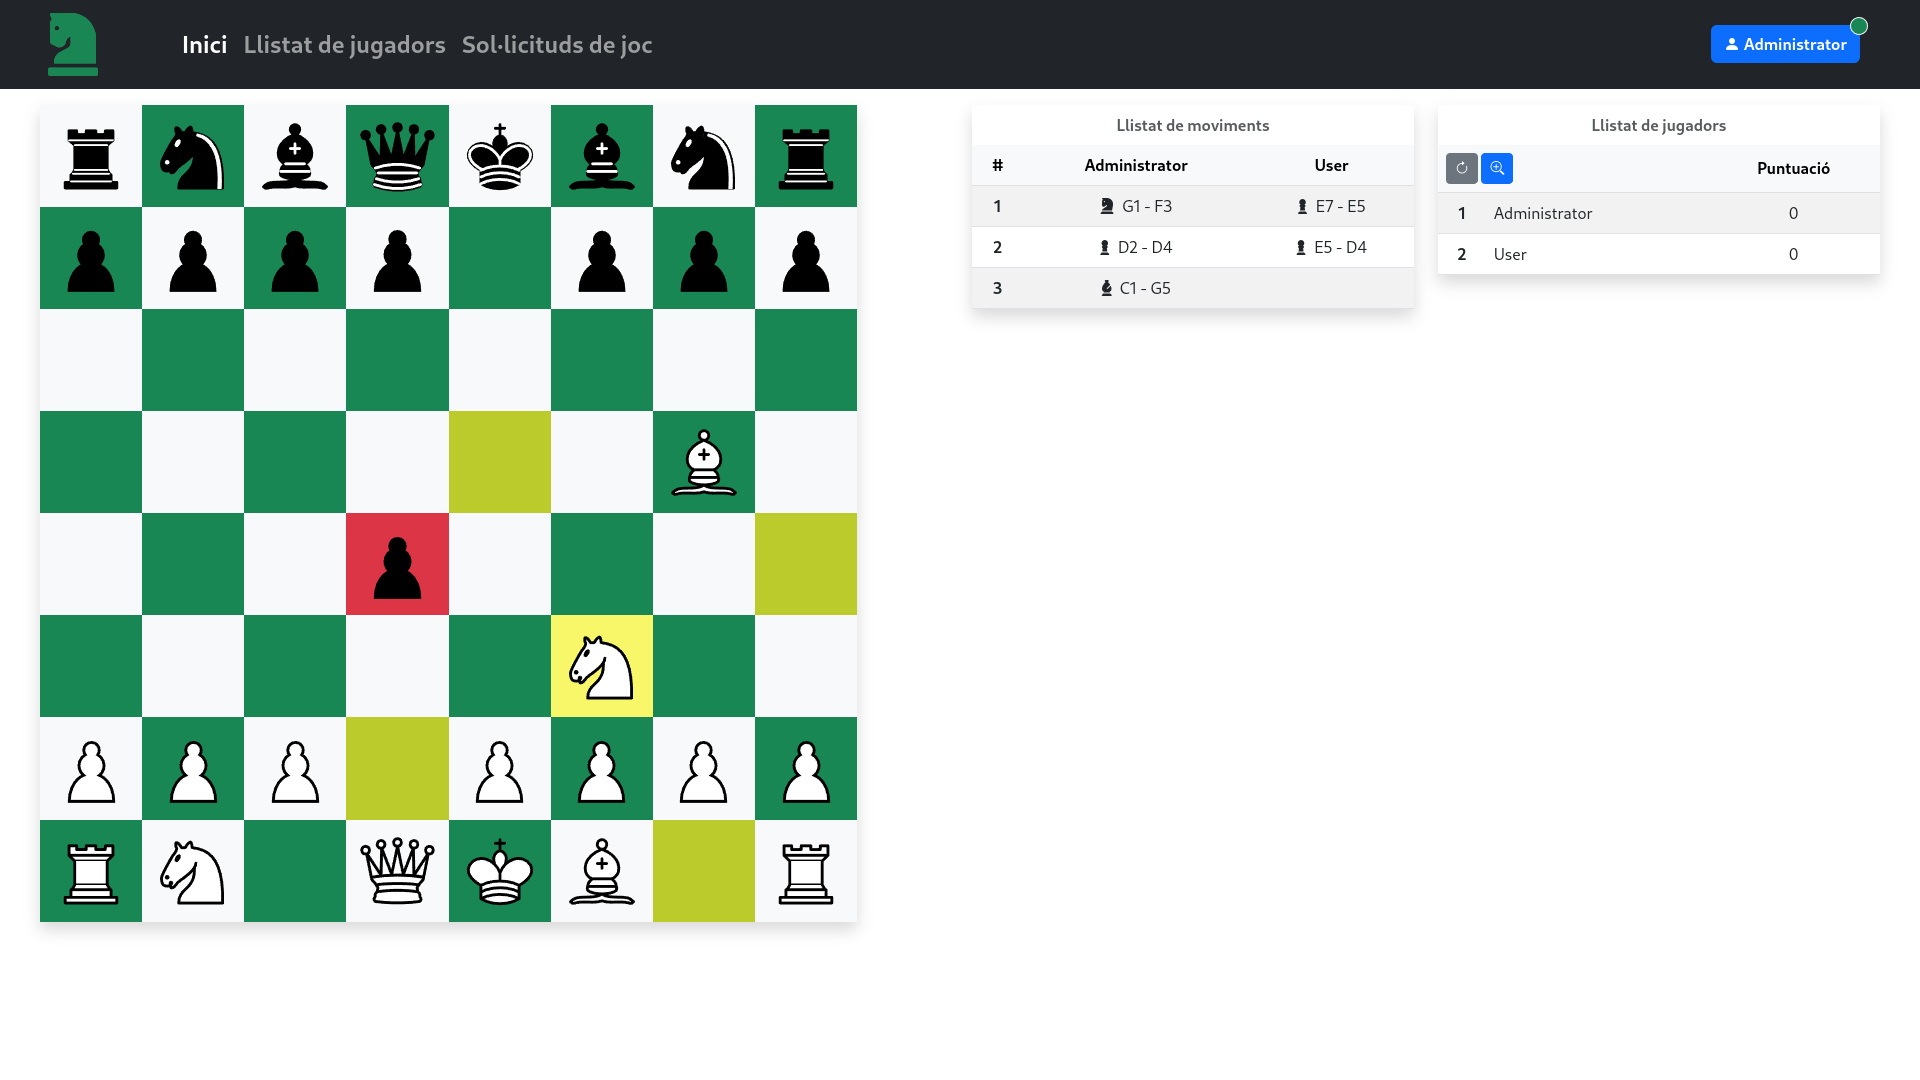
\includegraphics[width=0.8\textwidth]{images/index-escacs.png}
    \caption{Captura de la pàgina principal}
    \label{fig:Captura de la pàgina principal}
\end{figure}
\noindent
Tant la pàgina "Llistat de jugadors" com la de "Sol·licituds de joc" compten amb taulers similars, ambdós estan subscrits a un flux de dades, per tant, es recarreguen de forma automàtica. També compten amb un filtre per a facilitar la cerca.
\begin{figure}[H]
     \centering
     \begin{subfigure}[b]{0.8\textwidth}
         \centering
         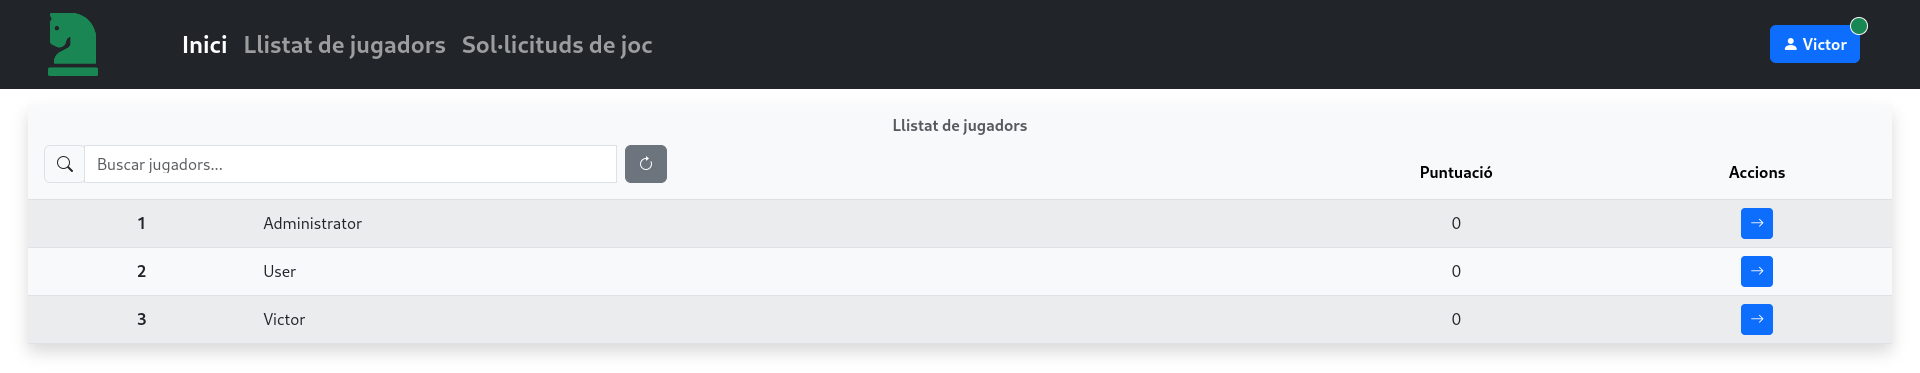
\includegraphics[width=\textwidth]{images/jugadors.png}
         \label{fig:Login}
     \end{subfigure}
     \begin{subfigure}[b]{0.8\textwidth}
         \centering
         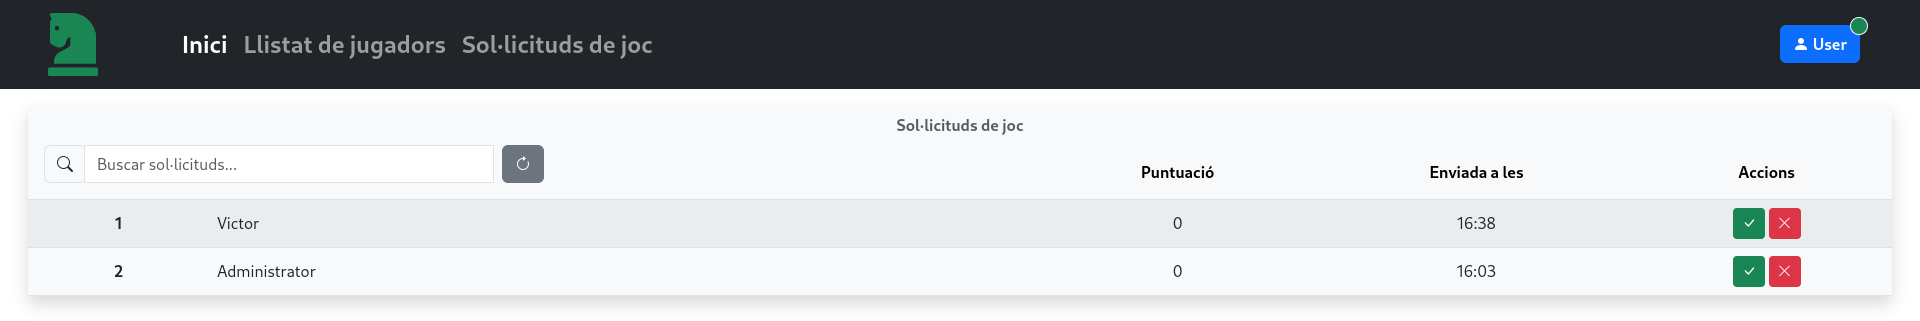
\includegraphics[width=\textwidth]{images/solicituds.png}
         \label{fig:Registre}
     \end{subfigure}
        \caption{Captures dels taulers de jugadors i sol·licituds}
        \label{fig:Captures dels taulers de jugadors i sol·licituds}
\end{figure}
\subsection{Persistència de dades rellevants a les partides}
La utilització d'un ORM simplifica molt aquest apartat, ja que no s'han descriure consultes SQL ni fer operacions de baix nivell de forma explícita. S'han definit diferents classes amb l'estereotip de repositori (anotació @Repository) que proporciona Spring Boot. Es poden observar al \hyperref[fig:Diagrama de classes de l'API]{diagrama de classes de l’API} a la secció "estructura de classes".
%-----------------------------------------------------------------------
\section{Proves}
Per a provar la part de la API s'han executat proves de tipus funcional mitjançant les ferramentes de depuració de Postman. Aquestes proves es centren en comprovar si el sistema compleix els requisits funcionals establerts, verificant que les funcionalitats del sistema funcionen com s'espera i produeixen els resultats correctes.
\\[3mm]
Postman és una plataforma de col·laboració i desenvolupament d'API que permet als desenvolupadors provar, depurar i documentar les seves API de manera eficient. És una eina molt utilitzada per enviar sol·licituds HTTP a les API, comprovar el seu funcionament i generar documentació interactiva.
\\[3mm]
El mòdul del motor d'escacs s'ha provat utilitzant proves d'unitat amb la ferramenta JUnit5. Aquestes proves es centren en comprovar el correcte funcionament de les unitats individuals del sistema. Es prova cada mòdul o component per separat per assegurar-se que funciona com s'espera i compleix les especificacions.
\\[3mm]
JUnit és un marc de proves unitàries per a Java que permet als desenvolupadors comprovar el comportament i la funcionalitat de les seves classes i mètodes de manera automatitzada. Proporciona anotacions i assertions per definir casos de prova i verificar els resultats esperats. JUnit és àmpliament utilitzat per assegurar la qualitat del codi i detectar errors.
\begin{figure}[H]
     \centering
     \begin{subfigure}[h]{0.5\textwidth}
         \centering
         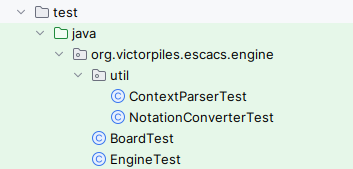
\includegraphics[width=\textwidth]{images/junit.png}
         \label{fig:Login}
     \end{subfigure}
     \hspace{0.10\textwidth}
     \begin{subfigure}[h]{0.35\textwidth}
         \centering
         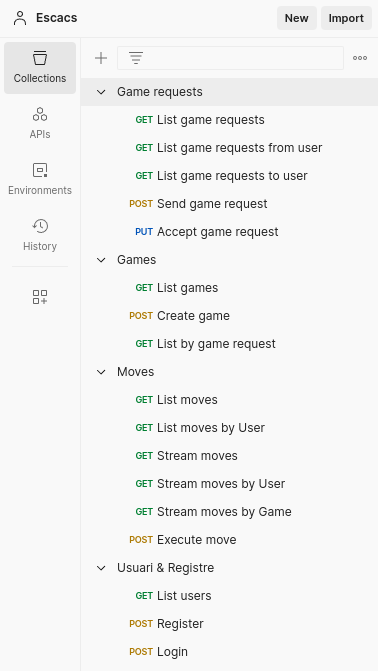
\includegraphics[width=\textwidth]{images/postman.png}
         \label{fig:Registre}
     \end{subfigure}
        \caption{Tests JUnit i Postman}
        \label{fig:Tests JUnit i Postman}
\end{figure}
%-----------------------------------------------------------------------
\section{Implantació i configuració}
En aquesta secció s'abordaran els passos necessaris per a la instal·lació, configuració i posada en marxa del software perquè pugui ser utilitzat a un entorn real. S'ha de tindre en compte que la forma de desplegar del servidor serà diferent a la del client, ja que utilitzen tecnologies diferents.
\subsection{Implantació del servidor: Maven Deploy i GitHub Packages}
El cicle de vida del codi del servidor s'ha gestionat amb Maven, aquesta és una eina utilitzada per construir i gestionar projectes de software, principalment en el llenguatge Java. Ajuda els desenvolupadors a gestionar les dependències del projecte (biblioteques externes i frameworks en què es basa el projecte) i a automatitzar el procés de construcció. També proporciona una estructura estàndard per organitzar el codi font i els recursos dels projectes.
\\[3mm]
Per a crear una nova versió en format JAR del projecte, s'ha configurat una acció de GitHub. Les accions de GitHub són una característica que permet automatitzar els fluxos de treball de desenvolupament en la plataforma GitHub. Permet configurar tasques automatitzades que s'executin en resposta a esdeveniments específics del repositori. Aquestes accions es defineixen en fitxers de configuració i poden incloure passos com la compilació, les proves i el desplegament del codi. Utilitzar les accions de GitHub millora l'eficiència, la qualitat del codi i facilita la col·laboració amb altres desenvolupadors.
\\[3mm]
En concret s'ha configurat una acció que, quan es publica una nova versió del programa a la secció "releases" del \href{https://github.com/VictoRPiles/escacs}{repositori de GitHub}, executa el comandament "maven:deploy" i després utilitza la configuració del pom.xml per a pujar el paquet al núvol de Maven i annexar-lo al repositori.
\\[3mm]
Per tant, per a utilitzar el servidor s'ha de descarregar el paquet al \href{https://github.com/VictoRPiles/escacs}{repositori de GitHub} i després simplement executar el JAR.
\begin{figure}[H]
    \centering
    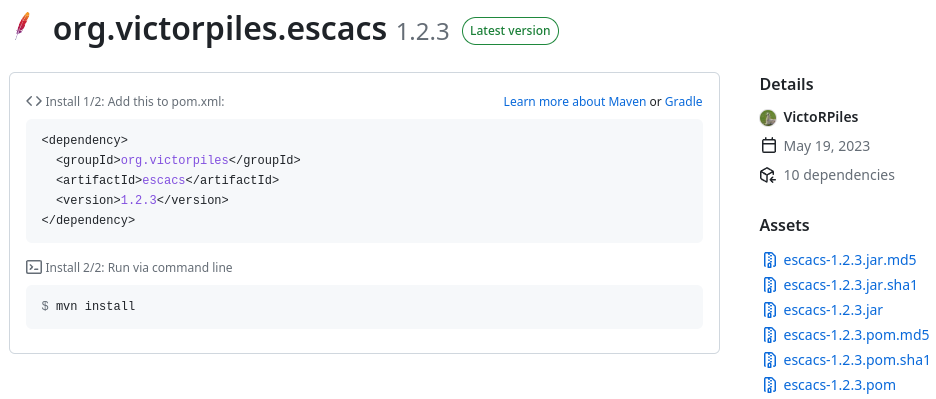
\includegraphics[width=\textwidth]{images/maven-publish.png}
    \caption{Paquet del servidor al \href{https://github.com/VictoRPiles/escacs}{repositori de GitHub}}
    \label{fig:Maven Deploy i GitHub Packages}
\end{figure}
\subsection{Implantació del client: Node Package Manager i Electron Forge}
Per a la gestió de dependències i cicle de vida del codi al client, s'ha utilitzat el sistema de gestió de paquets de NodeJS, anomenat npm (Node Package Manager), que ofereix una àmplia varietat de mòduls i llibreries predefinits per a la construcció d'aplicacions web.
\\[3mm]
Per a empaquetar l'aplicació com un executable, s'ha utilitzat Electron Forge, aquesta és una eina per empaquetar i distribuir aplicacions Electron. Combina molts paquets d'ús específic per crear un flux de construcció que funciona amb poca configuració, inclou signatura de codi, instal·ladors i publicació d'artefactes. Per a fluxos de treball avançats, es pot afegir lògica de construcció personalitzada en el cicle de vida de Forge mitjançant la seva API de connectors. Les destinacions personalitzades de construcció i emmagatzematge es poden gestionar configurant els "Makers" i "Publishers".
\\[3mm]
Per a crear un instal·lador, específic per al sistema operatiu amfitrió, s'ha d'executar el comandament "npm run make", després s'ha d'instal·lar (doble clic en Windows o utilitzant el gestor de paquets a Linux i MacOS).
\begin{figure}[H]
     \centering
     \begin{subfigure}[b]{0.4\textwidth}
         \centering
         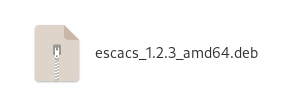
\includegraphics[width=\textwidth]{images/npm-make-deb.png}
         \label{fig:Alfil}
     \end{subfigure}
     \hspace{0.15\textwidth}
     \begin{subfigure}[b]{0.4\textwidth}
         \centering
         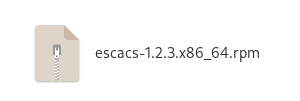
\includegraphics[width=\textwidth]{images/npm-make-rpm.png}
         \label{fig:Rei}
     \end{subfigure}
        \caption{Client empaquetat per a Debian i Fedora Linux}
        \label{fig:Desplaçament vectorial i no vectorial}
\end{figure}